\documentclass[a4paper]{article}

\usepackage{graphicx} % Required for inserting images

\begin{document}
\begin{titlepage}
\begin{center} 

        \Huge{Report} \vspace{1cm} 
        
        \large{Pooja Yakkala} \vspace{0.3cm}
        
        
    \end{center} 
\end{titlepage} 

To get started with building a decision tree, I imported a few important packages such as numpy, pandas, and graphviz. Then I initialized the decision tree node with the basic attributes that I know it will have such as attribute names, threshold value, left subtree and right subtree, value of the node as well as the gain computed. Then I proceeded to create a Decision Tree class which builds the tree by finding the computation of either the Gini Index or Information Gain, finding the best attribute using that computation, splitting the dataset into a left subtree dataset and right subtree dataset, finding the value of the leaf nodes, predicting the class and finally representing the tree in graphviz. I have also included the randomsplit function which ensures that the randomness of the data split is in check. (Although the data was already given after splitting, in case of a real-world scenario this would benefit by bringing in consistency.) The user gets to input either “gini or “entropy” and the model computes the gini/entropy of each attribute finds out the best attribute and splits the dataset based on it. Upon training the model using a custom fit() function, we calculate the accuracy, precision, recall, f1 score, specificity, false positive rate, false negative rate, and negative predictive value. The tuning process in the code is a brute-force method that checks which node-splitting criteria is the best. Then I reran the model with new parameters and compared the accuracies of both the Gini Index and Information Gain.

\section*{Any challenges faced}

When I was building my tree, I accidentally assigned the dataset of the left subtree to the right so my tree was visualized on the opposite side and my accuracy fell to 0.32 (32 percent). The next one was when I was comparing Gini Index and Information Gain with the trivial majority class classifier, I faced difficulty while computing the accuracy. As I was only performing the flatten function on one of the inputs (ypred), the other input was of a different dimension, and when I was computing accuracy I was getting 71 instead of a value between 0 and 1. The other challenge I faced was the same accuracy values for Gini as well as information gain. So, I thought that my calculations were going wrong because I had somewhat similar trees with one or two features different. The last one was when I was trying to draw the tree diagram, the graphviz was not working and I was getting an error to make sure I had graphviz executable in my computer which I did via Python.

\section*{How we overcome this}
For the first challenge, I corrected my assigned values and reran the model to make sure the tree was printed as it was originally. For the second challenge, I flattened both ytrue (the actual y values) and ypred (the predicted y values and checked the accuracy which now returned to a value between 0 and 1. For the third challenge, I learned that the values of Gini and Information gain are computed similarly and give almost the same best attributes hence the decision trees are similar but not the same. For the last challenge, I found out through Stackoverflow that I had to install the exe from the website and set a path for that on my computer.

\section*{Observations and Reference}
This paper talks about an image processing technique that is used for detecting malignant cells for breast tumors. The method they proposed helps physicians diagnose breast tumors by using techniques such as linear programming-based inductive classifiers and active countermodels such as snakes. The key points that I observed in this paper are the interactive graphical interface and the accuracy of this model. Many medical professionals and physicians may not be experts in using advanced machine learning and image-processing models.  By introducing a user-friendly interface, the model is made simple to use by any untrained observers, which is a positive point. I also appreciate the fact that they obtained the ten-fold cross-validation accuracy of 97 percent by using a single separating plane on three of the thirty features, which represents a notable best diagnostic result in the literature of medicine. Moreover, the use of the snakes method helped in minimizing the energy function of the arclength of a closed curve, which as a result marked the boundaries of the nuclei in cells precisely. This paper also predicted distant recurrence of malignancy in patients with an accuracy of 86 percent which is impressive. 
Along with all the strengths, I also think that there are certain limitations in this paper. The authors mentioned that they used MSM-Tree to minimize the misclassified points by recursively constructing a plane that minimizes the average distance of misclassified points to the plane. To stop the recursion, they didn't use pruning even though the algorithm has it but they manually restricted the number of separating planes to minimize the number of decision areas. This could have been better if the model had automated the pruning. One other drawback is that this model also requires fairly precise initialization to converge to a desired contour. Moreover, the feature set of this model is not broad. Including new features may help in making this model best suited for analysis of other diseases as well.

\section*{Performance results on the test set in a five-column table with accuracy, error, precision, and recall, using rows for Gini and IG, respectively.}
As shown in the table, the metrics for Gini and Information Gain are similar for the training dataset. The only difference between Gini and Information Gain is that with binary classification, Gini Index is preferred over information gain because it is more computationally efficient while entropy is preferred when there is a dataset imbalance. Comparing these two when tested with the test dataset, we can see that there is a difference between them, with Gini index accuracy at 0.929825 and Information Gain at 0.956140. Comparing these with a trivial majority class classifier, we can see that the majority classifier produces inaccurate results by labeling all of the data with the majority class. The accuracy stands at 0.622807.
\newpage
\begin{figure}
    \centering
    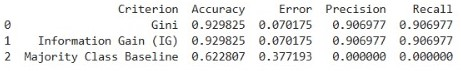
\includegraphics[width=0.5\linewidth]{table.jpg}
    \caption{Q7}
    \label{fig:enter-label}
\end{figure}

\section*{If precision or recall is most critical (most important) as a performance metric for this problem.}
If we think of having breast cancer as a positive case, then recall is the most critical performance measure. Recall which is also known as sensitivity focuses on identifying all positive cases. That is, it focuses on minimizing false negatives/missed positive cases. Getting a positive when the true value is negative (Doesn’t have cancer) doesn’t make much difference but getting a negative for a positive is dangerous, especially in medical disease identification. Precision however focuses more on minimizing false positives which is not very relevant in a medical context unless we perceive the case as - having breast cancer as negative and not having as positive.

\section*{Tuning procedure with the dev (tuning) set and what we learned from this part of the problem.}
For tuning my decision tree, I have used the brute-force method by looping with max-depth and mode. I have taken a set of max-depths = [3, 5, 7, 15, 20, 25] and mode as either ‘gini’ or ‘entropy’. As the loop runs, the parameters for each tree are added to a dictionary. Then we find the best hyperparameters out of that dictionary. For me, the best hyperparameters turned out to be max-depth = 5 and mode = ‘entropy’ for information gain and max-depth = 7 and mode = ‘gini’ for Gini Index. After performing tuning with the Chi-square test, I have found that there is a difference between active and inactive state accuracy's With the best hyperparameters, we can get increased accuracies by choosing the best node-splitting technique.

\section*{The decision-tree visualization}
\newpage
\begin{figure}
    \centering
    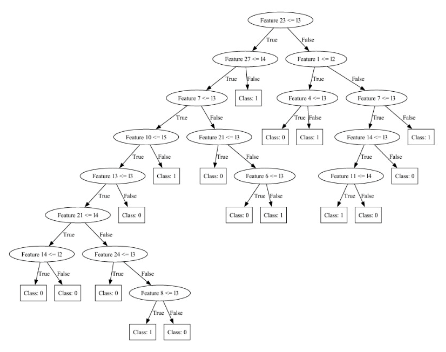
\includegraphics[width=0.5\linewidth]{dt.PNG}
    \caption{Q10}
    \label{fig:enter-label}
\end{figure}

\section*{Best-performing informativeness metric compared with the best-performing result in the experiment.}
As recall is the critical metric used in the given case of the breast cancer dataset, if we consider it as the best-performing metric, then we can say that the Information Gain model has the best result of 0.928571 as compared to Gini which has 0.880952 or Majority Class Classifier which has 0.0. However, if we consider accuracy as the best-performing metric, we can see that Information Gain is still the best-performing metric compared to the other two. In chi-square testing, when the chi square is active the accuracy is 92 percent when it is inactive the value is 62 percent.

\section*{The similarities and differences between the implementation and that of scikit-learn.}
The similarities between my implementation and the scikit-learn implementation given are the choice of hyperparameters which include max-depth and criterion. And the best parameters turned out to be of the “information gain model” in both implementations with a slight difference in the max-depths. The major differences I observed are that in the implementation, they used Grid Search CV which identifies the areas of the search space that deserve more attention for the possible best parameters while I used a simple for loop which is computationally heavy and slower. The decision trees (features and their thresholds) are also quite different from what I got and what is present in the implementation. The accuracy for the implementation is 0.96 which shows that it is a good model while the accuracy of my implementation is not the best, it is not the worst as well.


\section*{The performance of the binned versus non-binned (normalized) data}
The accuracy of the model tested with non-binned data with the information gain model is 0.956140 and the model with the binned data is 0.977238. There is a difference in the accuracy of binned and non-binned data. Here binned data is more accurate than non-binned data. Same with the precision and recall which are better for the binned data.

\section*{Speculating why that may be.}
In the binned dataset, the data is classified into 6 bins from l1 to l6. Binning makes it easier for algorithms to learn especially for algorithms that work on categorical features such as decision trees. It generalizes data into broad categories so there is little room for overfitting. While the non-binned dataset aka normalized data date scaled down to cover a certain range. It preserves even the smallest information in the data. Especially in the case of decision trees with categorical values, binned data performs better because this way the tree can split more easily than ones with normalized data where finding thresholds is a lot harder. The number of splits over the values is also reduced because there are no continuous values for which we find unique values to split with, they are already specified.

\section*{Observations}
min-samples-split and min-samples-leaf are the two additional categories that I find very useful. For min-samples-split, it means the minimum number of samples required to split the internal node. Increasing this value makes the model have larger leaf nodes and prevents overfitting. This also reduced the complexity of the decision tree for large datasets. Looking at the tree diagrams online that used min-samples-split, we can observe that trees with low min-samples-split can overfit the data while trees with higher min-samples-split can underfit the data. With min-samples-leaf, it controls the minimum number of samples required to be at a leaf node. It ensures that each node has enough data to make a good decision. It also prevents overfitting to noise or outliers.

\end{document}
